%Version 3.1 December 2024
% See section 11 of the User Manual for version history
%
%%%%%%%%%%%%%%%%%%%%%%%%%%%%%%%%%%%%%%%%%%%%%%%%%%%%%%%%%%%%%%%%%%%%%%
%%                                                                 %%
%% Please do not use \input{...} to include other tex files.       %%
%% Submit your LaTeX manuscript as one .tex document.              %%
%%                                                                 %%
%% All additional figures and files should be attached             %%
%% separately and not embedded in the \TeX\ document itself.       %%
%%                                                                 %%
%%%%%%%%%%%%%%%%%%%%%%%%%%%%%%%%%%%%%%%%%%%%%%%%%%%%%%%%%%%%%%%%%%%%%

%%\documentclass[referee,sn-basic]{sn-jnl}% referee option is meant for double line spacing

%%=======================================================%%
%% to print line numbers in the margin use lineno option %%
%%=======================================================%%

%%\documentclass[lineno,pdflatex,sn-basic]{sn-jnl}% Basic Springer Nature Reference Style/Chemistry Reference Style

%%=========================================================================================%%
%% the documentclass is set to pdflatex as default. You can delete it if not appropriate.  %%
%%=========================================================================================%%

%%\documentclass[sn-basic]{sn-jnl}% Basic Springer Nature Reference Style/Chemistry Reference Style

%%Note: the following reference styles support Namedate and Numbered referencing. By default the style follows the most common style. To switch between the options you can add or remove “Numbered” in the optional parenthesis. 
%%The option is available for: sn-basic.bst, sn-chicago.bst%  
 
%%\documentclass[pdflatex,sn-nature]{sn-jnl}% Style for submissions to Nature Portfolio journals
%%\documentclass[pdflatex,sn-basic]{sn-jnl}% Basic Springer Nature Reference Style/Chemistry Reference Style
\documentclass[pdflatex,sn-mathphys-num]{sn-jnl}% Math and Physical Sciences Numbered Reference Style
%%\documentclass[pdflatex,sn-mathphys-ay]{sn-jnl}% Math and Physical Sciences Author Year Reference Style
%%\documentclass[pdflatex,sn-aps]{sn-jnl}% American Physical Society (APS) Reference Style
%%\documentclass[pdflatex,sn-vancouver-num]{sn-jnl}% Vancouver Numbered Reference Style
%%\documentclass[pdflatex,sn-vancouver-ay]{sn-jnl}% Vancouver Author Year Reference Style
%%\documentclass[pdflatex,sn-apa]{sn-jnl}% APA Reference Style
%%\documentclass[pdflatex,sn-chicago]{sn-jnl}% Chicago-based Humanities Reference Style

%%%% Standard Packages
%%<additional latex packages if required can be included here>

\usepackage{graphicx}%
\usepackage[T2A]{fontenc}   % Cyrillic font encoding
\usepackage[utf8]{inputenc} % Encoding for source files (UTF-8)
\usepackage[russian]{babel} % Language support for Russian
\usepackage{multirow}%
\usepackage{amsmath,amssymb,amsfonts}%
\usepackage{amsthm}%
\usepackage{mathrsfs}%
\usepackage[title]{appendix}%
\usepackage{xcolor}%
\usepackage{textcomp}%
\usepackage{manyfoot}%
\usepackage{booktabs}%
\usepackage{algorithm}%
\usepackage{algorithmicx}%
\usepackage{algpseudocode}%
\usepackage{listings}%
%%%%

%% as per the requirement new theorem styles can be included as shown below
\theoremstyle{thmstyleone}%
\newtheorem{theorem}{Theorem}%  meant for continuous numbers
%%\newtheorem{theorem}{Theorem}[section]% meant for sectionwise numbers
%% optional argument [theorem] produces theorem numbering sequence instead of independent numbers for Proposition
\newtheorem{proposition}[theorem]{Proposition}% 
%%\newtheorem{proposition}{Proposition}% to get separate numbers for theorem and proposition etc.

\theoremstyle{thmstyletwo}%
\newtheorem{example}{Example}%
\newtheorem{remark}{Remark}%

\theoremstyle{thmstylethree}%
\newtheorem{definition}{Definition}%

\raggedbottom
%%\unnumbered% uncomment this for unnumbered level heads

\begin{document}

\title[Habiteer: мобильное приложение для формирования привычек]{Habiteer: мобильное приложение для формирования привычек}

%%=============================================================%%
%% GivenName	-> \fnm{Joergen W.}
%% Particle	-> \spfx{van der} -> surname prefix
%% FamilyName	-> \sur{Ploeg}
%% Suffix	-> \sfx{IV}
%% \author*[1,2]{\fnm{Joergen W.} \spfx{van der} \sur{Ploeg} 
%%  \sfx{IV}}\email{iauthor@gmail.com}
%%=============================================================%%

\author{\fnm{Артем} \sur{Дементьев}}

\affil{\orgdiv{Санкт-Петербургская школа физико-математических и компьютерных наук}, \orgname{НИУ ВШЭ в Санкт-Петербурге}, \orgaddress{\city{Санкт-Петербург}, \country{Россия}}}

\abstract{Многие люди стремятся формировать полезные привычки и избавляться от вредных, но сталкиваются с трудностями из-за недостатка мотивации, сложности внедрения изменений и ограниченности силы воли. Существующие приложения для отслеживания привычек...

Цель работы — разработать прототип мобильного приложения для проверки эффективности метода ««Tiny Habits»» в формировании привычек.

Приложение Habiteer, основанное на методе «Tiny Habits», позволит пользователям эффективнее формировать привычки за счет минимизации усилий и интеграции в повседневную жизнь. Результаты тестирования покажут, что Habiteer превосходит аналоги по уровню автоматичности формируемых привычек и удовлетворенности пользователей.}

%%================================%%
%% Sample for structured abstract %%
%%================================%%

% \abstract{\textbf{Purpose:} The abstract serves both as a general introduction to the topic and as a brief, non-technical summary of the main results and their implications. The abstract must not include subheadings (unless expressly permitted in the journal's Instructions to Authors), equations or citations. As a guide the abstract should not exceed 200 words. Most journals do not set a hard limit however authors are advised to check the author instructions for the journal they are submitting to.
% 
% \textbf{Methods:} The abstract serves both as a general introduction to the topic and as a brief, non-technical summary of the main results and their implications. The abstract must not include subheadings (unless expressly permitted in the journal's Instructions to Authors), equations or citations. As a guide the abstract should not exceed 200 words. Most journals do not set a hard limit however authors are advised to check the author instructions for the journal they are submitting to.
% 
% \textbf{Results:} The abstract serves both as a general introduction to the topic and as a brief, non-technical summary of the main results and their implications. The abstract must not include subheadings (unless expressly permitted in the journal's Instructions to Authors), equations or citations. As a guide the abstract should not exceed 200 words. Most journals do not set a hard limit however authors are advised to check the author instructions for the journal they are submitting to.
% 
% \textbf{Conclusion:} The abstract serves both as a general introduction to the topic and as a brief, non-technical summary of the main results and their implications. The abstract must not include subheadings (unless expressly permitted in the journal's Instructions to Authors), equations or citations. As a guide the abstract should not exceed 200 words. Most journals do not set a hard limit however authors are advised to check the author instructions for the journal they are submitting to.}

\keywords{keyword1, Keyword2, Keyword3, Keyword4}

%%\pacs[JEL Classification]{D8, H51}

%%\pacs[MSC Classification]{35A01, 65L10, 65L12, 65L20, 65L70}

\maketitle

\section{Введение}\label{Introduction}
\subsection{Актуальность}\label{Relevance}

Согласно Канеману (2011), человеческое мышление можно разделить на две системы: систему 1 и систему 2. Система 1 действует быстро и интуитивно, почти на автомате. Система 2, напротив, работает медленно и требует больше усилий. Она отвечает за сознательные умственные процессы, такие как анализ, принятие решений и самоконтроль. Однако ресурсы системы 2 ограничены — сила воли истощается в течение дня \cite{kahneman_thinking_2011}. Привычки помогают увеличить запас силы воли. Когда действие становится привычным, оно больше не требует активного контроля и выполняется на автомате, освобождая систему 2 для решения более сложных задач, таких как планирование или творчество.

Привычки во многом определяют нашу повседневную жизнь. Исследование Университета Дюка показало, что привычки составляют около 40-50\% ежедневных действий человека \cite{wood_habits_2002}. Гарднер и соавторы (2019) отмечали, что основанные на привычках вмешательства способствуют изменению поведения \cite{gardner_habit_2019}. Многие люди стремятся формировать полезные привычки и избавляться от вредных, чтобы улучшить разные стороны своей жизни — например, повысить работоспособность, лучше справляться со стрессом или поддерживать физическую форму. Однако на пути к этим целям часто возникают трудности из-за нехватки мотивации, сложности внедрения изменений и ограниченности силы воли \cite{gardner_making_2012, noauthor_what_nodate}.

Мобильные приложения имеют значительный потенциал для содействия в формировании привычек. Смартфоны повсеместны и доступны — ими пользуются около 60,5\% мирового населения \cite{gill_how_2025}. Смартфоны всегда под рукой, они предоставляют возможность вмешательства в любую минуту, когда это необходимо. Нативные мобильные приложения позволяют полноценно использовать возможности смартфона, такие как камера, GPS и другие датчики. Кроме того, нативные приложения  оптимизированы под конкретную операционную систему и могут работать в офлайн-режиме. Также приложения позволяют персонализировать опыт пользователя, предлагая индивидуальные рекомендации и настройки.

Популярность мобильных приложений для формирования привычек продолжает расти. В 2024 году рынок таких приложений оценивался в 11,42 миллиарда долларов, и ожидается, что в ближайшие годы он будет увеличиваться в среднем на 14,41\% в год \cite{httpswwweconmarketresearchcom_habit_nodate}. Несмотря на высокий потенциал этих приложений, исследования показывают, что их эффективность может значительно различаться, и многие из них не используют научно обоснованные подходы \cite{lally_how_2010, stawarz_beyond_2015}.

\subsection{Связанные работы}\label{Related Works}

С апреля 2024 по март 2025 года автор этой работы совместно с другим исследователем проводил систематический обзор рандомизированных контролируемых испытаний (РКИ). Обзор был посвящен оценке эффективности мобильных приложений для формирования привычек \cite{dementyev_impact_2025}. Всего рассматривалось 2363 статьи, из которых только 3 были признаны подходящими. Из обзора были сделаны следующие выводы:

\begin{enumerate}
    \item На сегодняшний день, нельзя доказать, что мобильные приложения для формирования привычек эффективны или неэффективны
    \item Объясняется это тем, что в научной среде крайне мало исследований на эту тему, а также тем, что результаты существующих исследований противоречивы
    \item В 2/3 подошедших исследованиях был малый размер выборки. В одном из исследований был обнаружен высокий риск искажений (с учетом того, что качество второго исследования не рассматривалось)
\end{enumerate}

Уже то обстоятельство, что в систематическом обзоре было найдено лишь три подходящих исследования, говорит о значительном пробеле в научных знаниях. Влияние специализированных мобильных приложений на формирование привычек почти не исследовано, несмотря на их большое количество и спрос на рынке.

Как уже упоминалось, большинство приложений не используют научно обоснованные подходы в формировании привычек \cite{stawarz_beyond_2015}. Между тем, известно несколько таких подходов. Перед тем как мы их рассмотрим, необходимо уточнить, что именно подразумевается под понятием «привычка».

Привычка — это процесс, при котором контекст автоматически вызывает определённое действие посредством активации ментальных ассоциаций «контекст–действие», сформированных за счёт предыдущего опыта выполнения этого действия \cite{gardner_habit_2019}. Формирование привычки — это сложный процесс, включающий многократное повторение поведения в стабильных условиях, что приводит к возникновению автоматических реакций на определённые внешние сигналы (стимулы) \cite{Lally01052013}. Из этих определений можно вывести то, что (1) привычка — это автоматическая реакция на некий стимул; (2) автоматизм реакции развивается благодаря многократному повторению поведения и (3) поведение должно повторяться в стабильной среде. Первое — это определение привычки, второе и третье — условия ее формирования. Зная условия, можно выделить несколько научных подходов, которые помогают их создать.

П. Голлвитцер предложил стратегию реализационных намерений (implementation intentions), суть которой состоит в формулировке четких правил формата «если — то» \cite{gollwitzer_implementation_1999}. Например: «Если прозвенит будильник в 7:00 (стимул), то я сразу начну делать зарядку (действие)». Реализационные намерения повышают частоту и автоматизм новых действий, способствуя формированию привычек — как в работе, так и в повседневной жизни \cite{Trenz2024Promoting, Holland2006Breaking, Wicaksono2019Using, VanTimmeren2022Instant, ADRIAANSE2011183, lally_2008, tam_2010}. Такой подход помогает обеспечить регулярное выполнение нужного поведения, пока оно не станет автоматическим \cite{Trenz2024Promoting, Holland2006Breaking, Wicaksono2019Using}. 

Стимулы бывают разных видов, но исследователи советуют привязывать новые действия к другим действиям, хорошо закрепленным в рутине \cite{judah_2012, BAYER2022101303, fiorella_2020}. Этот подход называется «habit stacking» или «anchoring» («якорение»), или «piggybacking» \cite{BUABANG202541, rd_what_2023, doi:10.1177/237946151600200109}. Якорение опирается на уже существующие нейронные связи и контекстные сигналы, чтобы новые действия было легче запомнить и выполнять \cite{verplanken_2005, zogg_2011, clear_how_2014}. У этого подхода есть преимущество перед напоминаниями. Эффективность и заметность напоминаний со временем угасают, при этом напоминания практически не помогают сделать поведение автоматичным, в отличие от действий, привязанных к существующим привычкам \cite{stawarz_beyond_2015}. Использование внешних стимулов в некоторых ситуациях осложняется негативными социальными факторами — например, стигматизацией или психологической нагрузкой, связанной с определёнными действиями. В Уганде люди с ВИЧ сталкивались с трудностями при формировании привычки регулярного приёма лекарств из-за стигмы — раскрытие своего ВИЧ-статуса могло угрожать не только ухудшением отношений с близкими и сообществом, но также домашним насилием и потерей работы \cite{Stecher2022Barriers}. В целом, результативность якорения подтверждалась рядом исследований \cite{fournier_2017, https://doi.org/10.1111/bjhp.12263, KELLER201753, Pimm01102016}, однако в эксперименте Келлера и коллег (2021) не обнаружилось различий в автоматичности поведения между теми, кто привязывал действия ко времени, и теми, кто привязывал действия к другим привычкам \cite{https://doi.org/10.1111/bjhp.12504}.

У реализационных намерений имеются и ограничения. Жёсткие правила «если-то» могут затруднить адаптацию при смене контекста, теряют свою результативность, когда поведение сложное \cite{VanTimmeren2022Instant}, а также не всегда способствуют формированию автоматизма \cite{Wicaksono2019Using}. При этом, если намерение слабое, подход почти не способствует выполнению поведения \cite{Prestwich01122003, doi:10.1177/0146167204271308}.

\begin{figure}[h]
  \centering
  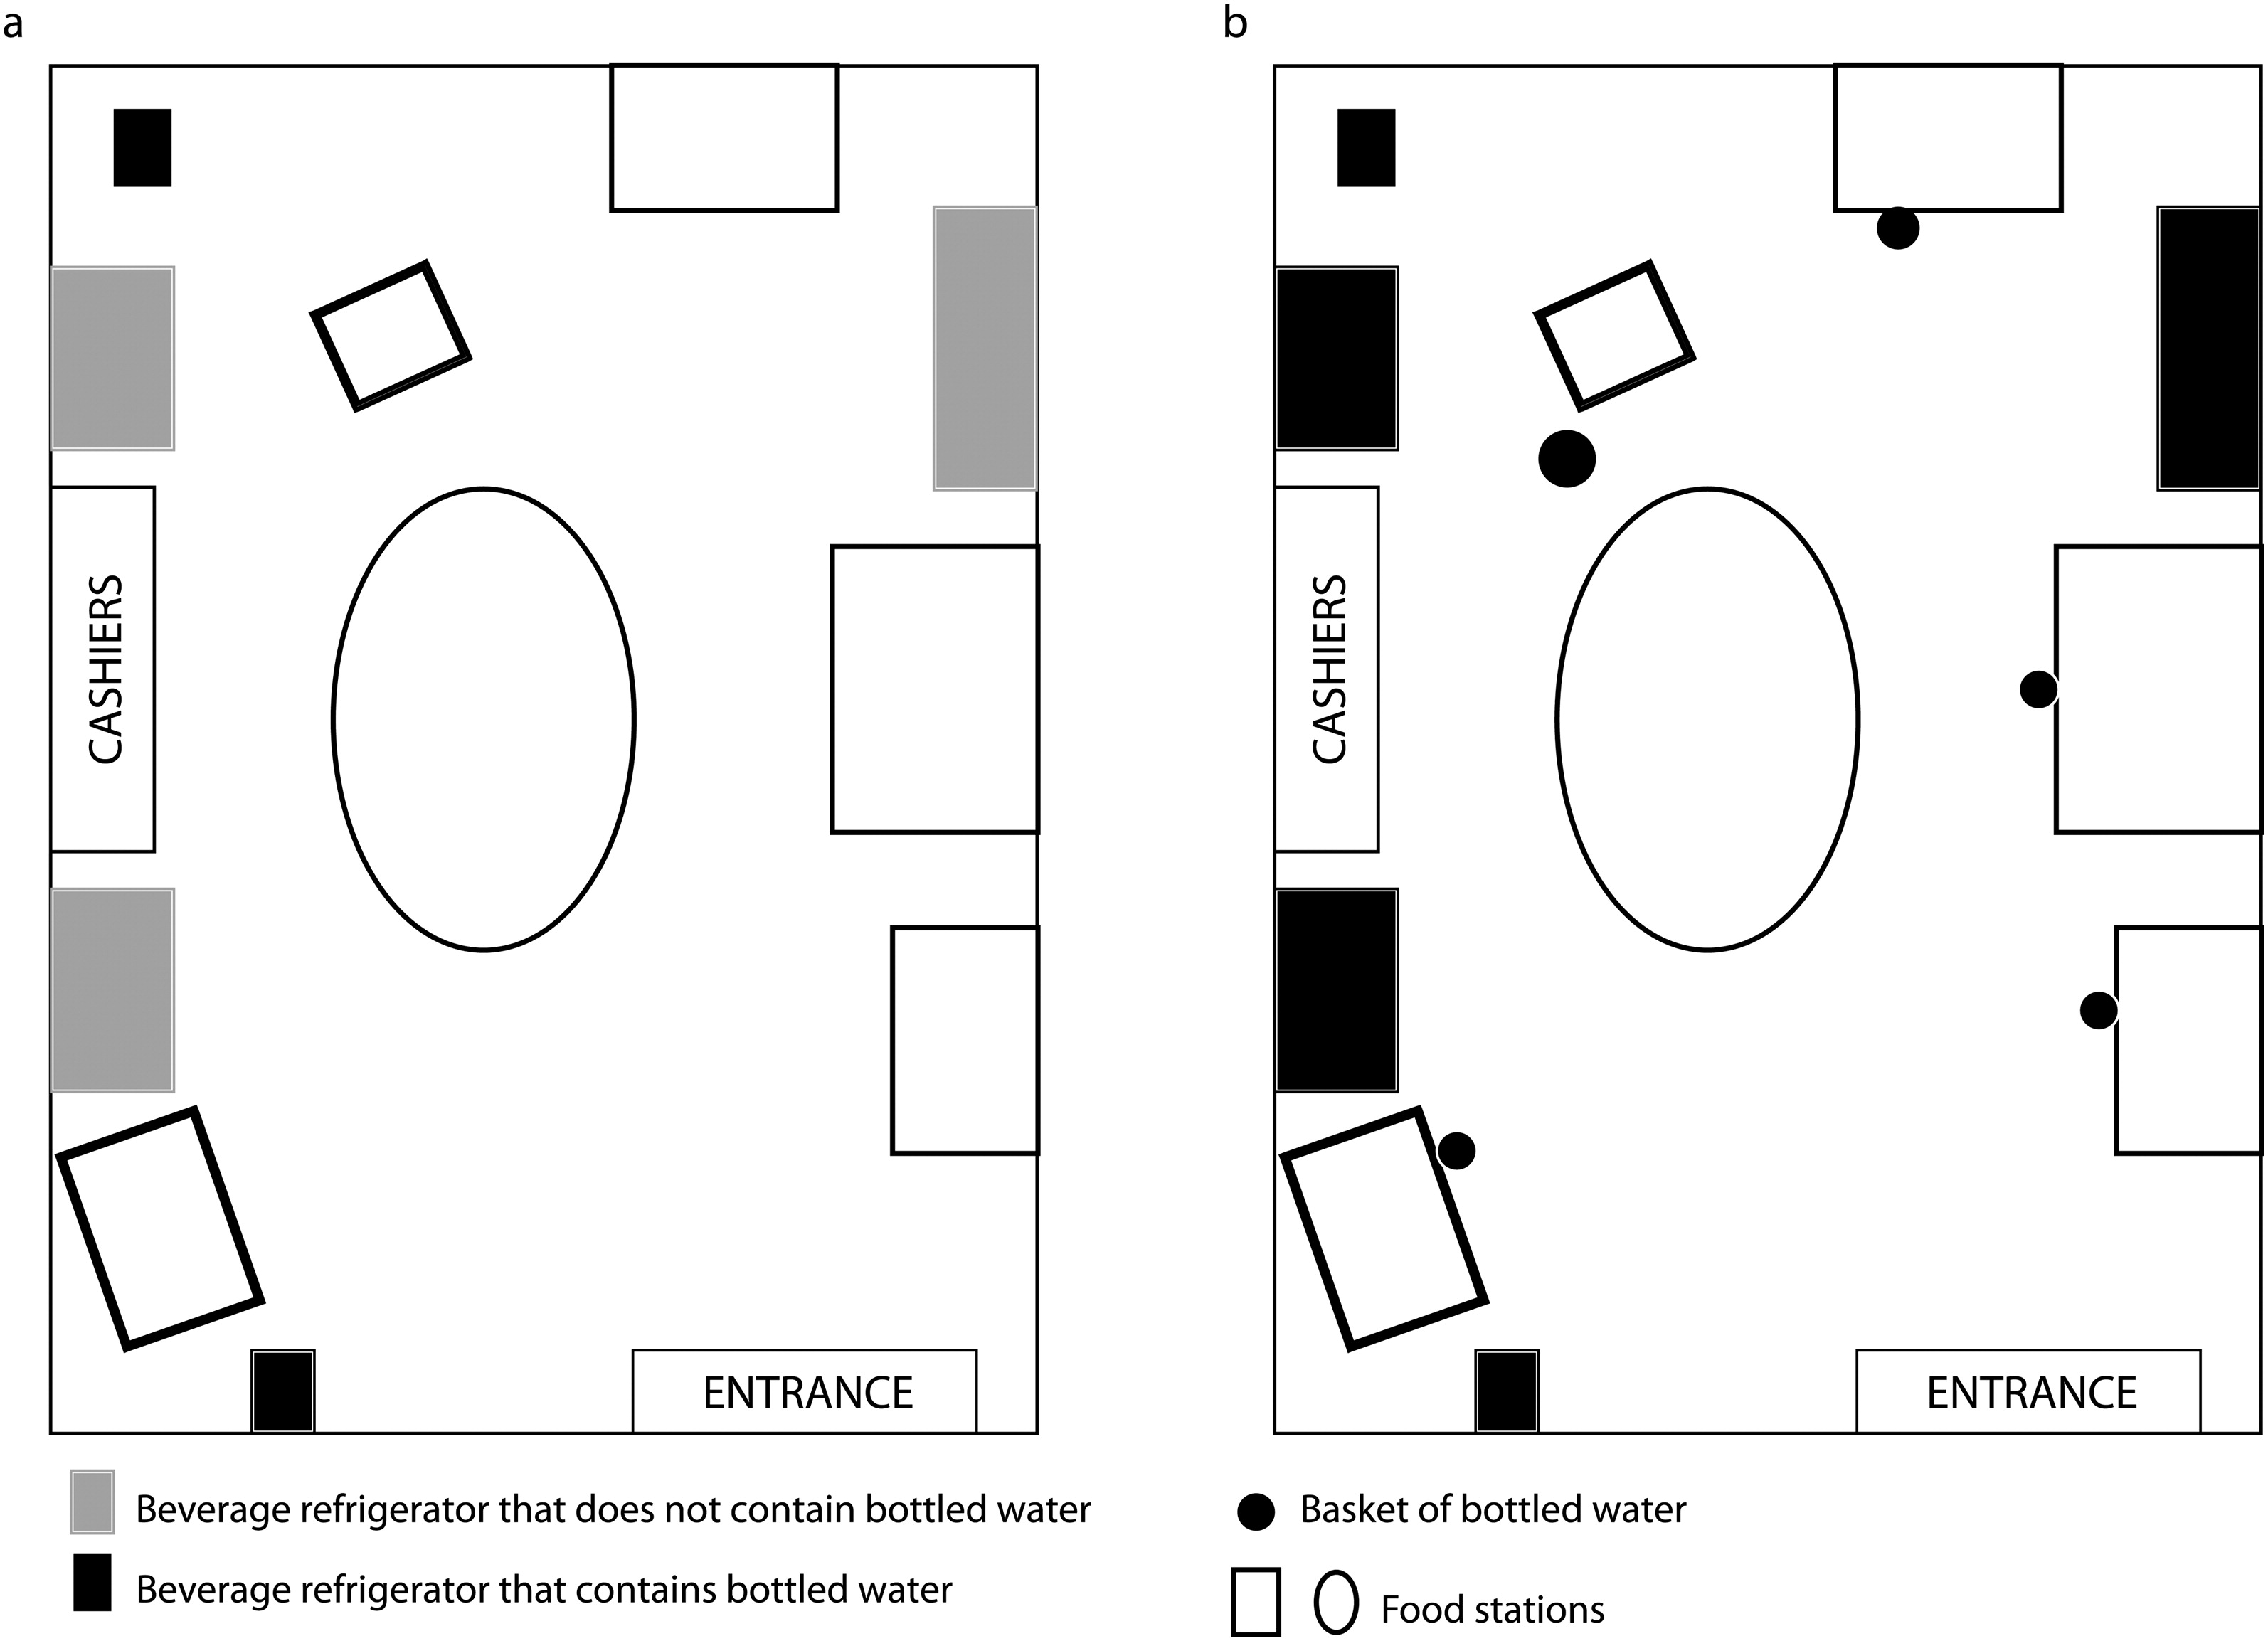
\includegraphics[width=\linewidth]{figures/thorndaik_architecture_choice.jpeg}
  \label{pic1}
  \caption{Картинка «a» показывает, как выглядело помещение до изменений, а картинка «b» — после изменений. Источник: American Journal of Public Health, April 2012}
\end{figure}

Эффективность формирования привычек также можно повысить с помощью «архитектуры выбора» («choice architecture»). Этот подход основан на управлении окружением и организации условий таким образом, чтобы предпочтительное поведение стало максимально лёгким и естественным, а нежелательное – наоборот, сложным и неудобным \cite{thaler_nudge_2008}. Торндайк и её команда провели исследование, чтобы изменить расположение продуктов в кафетерии больницы. Они начали с того, что добавили воду в холодильники, которые раньше были заполнены только газировкой, и поставили корзины с бутылками воды рядом с едой в разных частях кафе. Таким образом, вода стала доступна везде, где были напитки, в то время как газировка осталась в тех же холодильниках (рис. 1). Похожие изменения были внесены и в расположение еды. В результате продажа вредных напитков уменьшилась на 11,4\%, а продажа бутылок с водой увеличилась на 25,8\% \cite{thorndike_2012}.

Если реализационные намерения и архитектура выбора помогают связать поведение с контекстом, то позитивное подкрепление увеличивает вероятность, что поведение будет повторяться. Позитивное подкрепление (positive reinforcement) — это подход, основанный на принципах оперантного обусловливания, где поведение закрепляется за счёт последующего позитивного подкрепления – награды, одобрения или других приятных последствий \cite{Skinner1953}. Например, предоставление человеку награды после выполнения действия (даже символической, такой как похвала или отметка в дневнике достижений) существенно увеличивает вероятность повторения этого поведения в будущем. Удовольствие и внутренняя мотивация не только побуждают людей повторять нужное поведение, но и делают каждое повторение более эффективным для формирования привычки \cite{Landry2019Positive}. Этот эффект наблюдается в различных видах активности — от использования зубной нити и приёма витаминов до физических упражнений \cite{Judah2018Exploratory, Fremling2025Comparing, Wiedemann2014Intrinsic}.

Вышеперечисленные подходы в той или иной мере действенны и используются на практике. Есть и другие подходы, которые автор не стал упоминать из-за того, что они не так часто применяются в формировании привычек. Например, в таксономии техник изменения поведения насчитывается 93 техники, объединенных в кластеры \cite{michie_2008_bct}. Также имеется более современная версия таксономии с 281 техникой \cite{ontology_bct}. Каждая из этих техник теоретически может быть применена для формирования привычек, поскольку привычка — это вид поведения. Тем не менее, в научных исследованиях, посвященных формированию привычек, эти техники упоминаются достаточно редко.

Автор также обошел стороной теории изменения поведения и формирования привычек, такие как теория самодетерминации, модель COM-B, поведенческая модель Фогга, Habit Loop, теория запланированного поведения, транстеоретическая модель и прочие. Для понимания процесса формирования привычек подобные теории несомненно важны. Но для непосредственно создания привычек вряд ли эти теории более полезны, чем практические подходы и методы. Это подобно тому, как если бы кондитер вместо того, чтобы испечь торт по рецепту, стал бы часами изучать теорию приготовления пищи. Возможно, он смог бы создать свой рецепт на основе теоретических сведений о продуктах питания, но на это пришлось бы затратить больше усилий и времени, при этом никто не гарантирует, что торт, испеченный по собственному рецепту, окажется вкусным. В рамках данной работы интересны именно «рецепты» и то, насколько хороший результат можно с их помощью получить. Основные теории подробно описаны в работе К. Пиндера и соавторов, где рассматривается их применение к формированию привычек с использованием цифровых инструментов \cite{10.1145/3196830}.

Особенность рассмотренных подходов состоит в том, что они известны, как правило, в научной и «околонаучной» среде. На взгляд автора, это связано с тем, что эти подходы кажутся довольно «точечными», и мало известно о том, как они связаны с другими подходами, не говоря уже о том, чтобы они были увязаны в некий единый и понятный для широкой публики алгоритм. Ситуация с теориями еще сложнее, поскольку часто неясно, как применять их на практике. Это замечание особенно справедливо для описательных теорий, таких как теория самодетерминации, и менее справедливо для процедурных теорий, таких как модель Фогга или COM-B.

Наиболее известны три попытки популяризации поведенческой науки о формировании привычек для широкого круга читателей.

Первое издание «The Power of Habit» было опубликовано в 2012 году. Автор Чарльз Дахигг — журналист, а не эксперт в области нейробиологии или психологии, однако его модель Habit Loop обрела широкую известность, в том числе и в научной среде. Согласно этой модели, привычка формируется через цикл из трёх компонентов: сигнала (cue), поведения (routine) и вознаграждения (reward) \cite{duhigg_power_2012}. Важным дополнением к этому циклу является компонент «craving» (желание), который Дахигг вводит между сигналом и поведением. Это ощущение ожидания удовольствия, которое возникает в ответ на сигнал и предшествует выполнению рутинного действия. Процесс работает следующим образом: сигнал запускает желание (craving), которое, в свою очередь, побуждает к выполнению действия (routine). Это поведение закрепляется за счёт вознаграждения, которое служит подтверждением правильности выбора. Многократное повторение цикла способствует укреплению нейронных связей и закреплению привычки. Основная мысль — создать цикл, в котором сигнал запускает рутину, которая затем подкрепляется наградой. Несмотря на подробное и понятное описание процесса формирования привычек, в книге немного практических рекомендаций по внедрению этой модели в повседневную жизнь.

Широкую популярность получила книга «Atomic Habits» Дж. Клира, опубликованная в 2018 году, которая в том же году стала международным бестселлером \cite{noauthor_avery_nodate, editor_james_2022, bureau_james_nodate}. В отличие от «The Power of Habit», эта книга ориентирована на практическое применение принципов формирования привычек. В ней предлагаются четыре «закона» создания привычек: сделать поведение очевидным, привлекательным, легким и приятным \cite{clear_atomic_2018}. Можно сразу заметить, что эти четыре закона соответствуют циклу привычки Дахигга «cue-craving-routine-reward». Клир встраивает в этот цикл уже упомянутые выше научные подходы — реализационные намерения, архитектуру выбора, позитивное подкрепление, якорение, а также некоторые техники изменения поведения вроде self-monitoring of behavior (BCT 2.3). Для долгосрочного закрепления привычек Клир предлагает формирование привычек, основанных на идентичности. Согласно этому подходу, наиболее устойчивые привычки возникают тогда, когда поведение связано с самоощущением человека и его идентичностью. Например, человек, который считает себя спортсменом, с большей вероятностью будет регулярно заниматься спортом, поскольку это поведение является частью его личной идентичности. На официальном сайте Дж. Клира есть ссылка на мобильное приложение «Atoms», которое основано на системе «Atomic Habits» \cite{noauthor_atoms_nodate}.

Метод «Tiny Habits» был разработан Б.Дж. Фоггом, специалистом по поведенческим наукам, и впервые был представлен в 2019 году в его книге «Tiny Habits: The Small Changes That Change Everything» \cite{phd_tiny_2020}. Однако сам метод начал развиваться гораздо раньше — Фогг изучал поведенческие изменения и психологию людей более 20 лет, прежде чем официально представил свою методику \cite{noauthor_tiny_nodate}. Основная идея заключается в том, чтобы выбирать маленькие, простые действия и связывать их с уже существующими привычками \cite{noauthor_bj_nodate}. В «Tiny Habits» используются те же научные подходы, что и в «Atomic Habits», однако способ их применения существенно различается.

Начнем с того, что в «Atomic Habits» практически не затрагивается вопрос выбора привычек. Подразумевается, будто человек уже заранее знает, какую привычку хотелось бы ему привить. В «Tiny Habits» первоочередное внимание уделяется не просто выбору подходящей привычки, а прояснению «стремления» (aspiration) — той цели, ради которой человек готов меняться. Далее предлагается «мозговой штурм», в ходе которого необходимо придумать как можно больше вариантов поведения для достижения стремления. Эти варианты сортируются по трем критериям: желания и возможности выполнять поведение, а также эффективности поведения в достижении стремления. Выбирается та привычка, которая наиболее удовлетворяет перечисленным критериям. Такой подход усиливает внутреннюю мотивацию, поскольку выбор основан на личной значимости и высокой воспринимаемой полезности.

Следующее отличие состоит в том, что «Atomic Habits» основан на модели Habit Loop, в то время как «Tiny Habits» основан на собственной поведенческой модели. Поведенческая модель Фогга состоит из трех компонентов: мотивация (motivation), способность (ability) и подсказка (prompt). Согласно модели, поведение происходит только тогда, когда вместе соединяются все эти три компонента \cite{fogg_2009}. Фогг рекомендует уделить особое внимание способности — сделать поведение настолько легким, насколько это возможно \cite{phd_tiny_2020}. Сложность поведения зависит от пяти факторов: время, деньги, физические усилия, ментальные усилия и соответствие текущей рутине. Чтобы сделать поведение проще, нужно сначала выяснить, какой или какие из этих факторов делают поведение сложным, а затем можно снижать значимость этих факторов тремя способами: развивая навыки, используя вспомогательные инструменты, либо максимально упрощая само действие. Последнего можно добиться, разбив действие на микрошаги (например, вместо пробежки просто надеть кроссовки) или уменьшив его объем (например, сделать 2 отжимания вместо 20). После того, как поведение упрощено, требуется выбрать подсказку с помощью якорения. К слову, метод якорения в контексте формирования привычек был разработан именно Фоггом на основе предыдущих исследований, о чем упоминает Дж. Клир в своем блоге и в примечаниях к «Atomic Habits» \cite{clear_how_2014, clear_atomic_2018}.

Другое отличие заключается в том, что «Tiny Habits» предлагает «репетиции». После определения целевого поведения и подсказки предлагается сознательно повторить действие 7-10 раз подряд. Например, для «рецепта» привычки «после того, как я встаю с кровати, я делаю два отжимания», алгоритм будет следующим: (1) сесть на кровать, (2) встать, (3) выполнить два отжимания, (4) мысленно похвалить себя — и повторить всю последовательность 7-10 раз. Репетиции укрепляют нейронные связи, тем самым поведение становится более автоматичным. Так повышается устойчивость привычки и облегчается её выполнение в дальнейшем.

\begin{figure}[h]
  \centering
  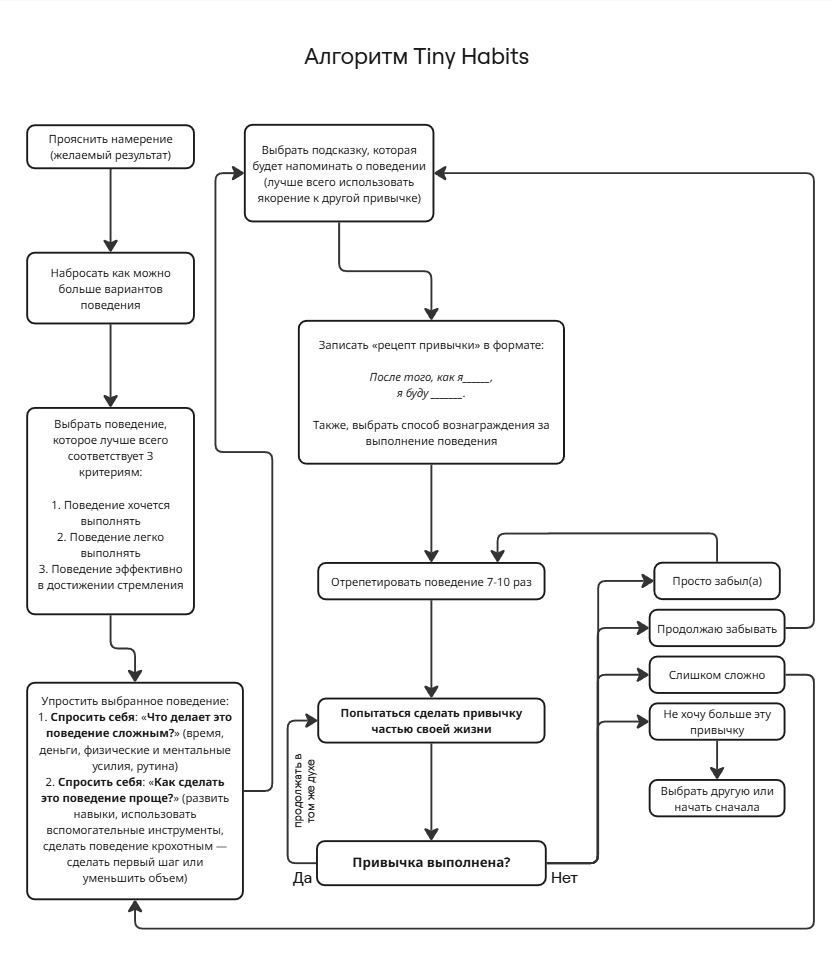
\includegraphics[width=\linewidth]{figures/tiny_habits_alg.jpg}
  \label{pic2}
  \caption{Алгоритм «Tiny Habits». Составлено автором по книге «Tiny Habits» (2020)}
\end{figure}

Метод «Tiny Habits» выделяется среди других методов и научных подходов своей ярко выраженной практической направленностью.  По мнению автора данной работы, советы и инструкции, представленные в «Tiny Habits», более последовательны и ясны, чем у других подходов. Именно этот метод предлагает конкретный и понятный алгоритм формирования привычек (рис. 2). Прочие подходы либо узконаправленные и затрагивают какой-то один аспект формирования привычек (например, реализационные намерения помогают соединить поведение с контекстом, а позитивное подкрепление выступает в роли катализатора), либо носят описательный характер (теории вроде Habit Loop), либо представляют собой перечень советов по формированию привычек (Atomic Habits).

Несколько исследований указывают на потенциальную эффективность метода «Tiny Habits» в формировании устойчивых привычек. Так, РКИ, посвященное влиянию «Tiny Habits» на благодарность, показало, что у участников, которые сосредоточились на культивировании благодарности с помощью маленьких привычек, значительно улучшились показатели самооценки благодарности, причем эффект сохранялся до одного месяца \cite{Hollingsworth2022Tiny}. Аналогично, пилотный эксперимент в области устойчивого потребления показал, что «Tiny Habits» способствует долгосрочному сохранению экологичных привычек \cite{OHalloran2024Small}. Еще одно исследование продемонстрировало эффективность поведенческих вмешательств, основанных на «Tiny Habits», для улучшения контроля за гликемией у пациентов с диабетом в Саудовской Аравии \cite{alqutub_2025}. Автору данной работы неизвестно о существовании других исследований, оценивающих эффективность метода «Tiny Habits», однако предыдущие работы показывают, что легковыполнимые действия с большей вероятностью становятся привычными \cite{lally_2010, https://doi.org/10.1348/014466605X49122}, так же, как действия, основанные на внутренней мотивации \cite{Judah2018Exploratory, phillips_2016}.

Хотя «Tiny Habits» показывает высокий потенциал в некоторых областях, его универсальность и долгосрочное влияние на различные типы поведения не доказаны. Кроме того, автор метода утверждает, что «Tiny Habits» был основан не столько на академической литературе, сколько на исследованиях самого автора \cite{tiny_habits_references}. Эти исследования являются частью курса Фогга «Tiny Habits», который был запущен в 2011 году, но при этом их результаты не были опубликованы. В настоящее время курс «Tiny Habits» проводится на коммерческой основе и название «Tiny Habits» является зарегистрированным товарным знаком \cite{noauthor_bj_nodate, noauthor_permissions_nodate}. Непрозрачность метода при довольно сильной коммерциализации лишний раз подчеркивает необходимость всесторонней оценки его эффективности.

\subsection{Обоснование значимости работы и ее цель}\label{Goal}

Пробел в научных знаниях и значимость данной работы можно сформулировать так.

Формировать полезные привычки важно, но в процессе люди часто сталкиваются с препятствиями. Для их преодоления существует множество подходов, из которых наиболее известны реализационные намерения, якорение, позитивное подкрепление и архитектура выбора. Эти подходы помогают связать целевое действие со стимулом (контекстом) и увеличить вероятность многоразового повторения этого действия в ответ на стимул, что, в итоге, должно привести к автоматической реакции — формированию привычки. Существуют также и методы, которые увязывают эти и другие подходы в некую систему. Наиболее известны две таких системы — «Atomic Habits» и «Tiny Habits», причем последняя примечательна своей исключительной практической направленностью и последовательностью. Несмотря на популярность метода и его высокий потенциал, эффективность «Tiny Habits» в формировании привычек почти не исследована. В качестве инструмента для вмешательств лучше всего подходят смартфоны из-за их распространенности, доступности и возможностей персонализации. Существует множество мобильных приложений по формированию привычек, однако их эффективность остается невыясненной и большинство из них не используют научные подходы и методы.

Таким образом, \textbf{цель работы} — разработать прототип мобильного приложения для проверки эффективности метода «Tiny Habits» в формировании привычек.

На основе прототипа разработчики смогут создать приложение, которое поможет:

\begin{enumerate}
    \item Отслеживать и формировать привычки (для конечных пользователей)
    \item Оценить эффективность метода «Tiny Habits» (например, с помощью экспериментов или анализа исторических данных)
    \item Оценить эффективность приложения как инструмента, содействующего в формировании привычек
\end{enumerate}

\textbf{Целевая аудитория приложения (ЦА)} — взрослые русскоговорящие пользователи, заинтересованные в саморазвитии и формировании привычек. К ЦА не относятся пользователи с серьезными зависимостями (например, табачной или наркотической), а также пользователи, которые желают значительных перемен в своем образе жизни. Причина исключения состоит в том, что первым требуется профессиональная помощь, а вторым необходимы более интенсивные вмешательства.

\subsection{Структура}\label{Structure}

Основная часть работы состоит из трех разделов: 1) контекст и потребности, 2) разработка решения, 3) итоговое оценивание. В начале каждого раздела ставятся исследовательские вопросы, выбираются подходящие методы для ответа на них, а в конце формулируются выводы и обозначаются ограничения. В заключительной части обсуждаются общие выводы, а также предлагаются практические рекомендации и дальнейшие направления исследований.

\newpage

\section{Контекст и потребности}\label{Context and Needs}

\subsection{Обзор раздела}\label{Overview1}

Люди пользуются продуктами и сервисами, когда эти продукты и сервисы удовлетворяют их потребности. Стало быть, прежде чем разрабатывать приложение, нужно выяснить, чего хотят люди и при каких обстоятельствах.

\bigskip
Исследовательские вопросы раздела:

\begin{itemize}
    \item В чем состоят характеристики целевой аудитории?
    \item Какие у нее потребности? При каких обстоятельствах эти потребности проявляются?
    \item Какие из этих потребностей наиболее важные?
    \item Что уже сделано для решения потребностей?
\end{itemize}

Исходя из исследовательских вопросов, были выбраны исследовательские методы и соответствующие UX-артефакты (см. таблицу \ref{tab:table1}).

\begin{table}[h]
\normalsize
\caption{Методы исследования, ключевые вопросы и артефакты}
\label{tab:table1}
\begin{tabular}{|l|p{5cm}|p{5cm}|}
\hline
\textbf{Метод}           & \textbf{Вопрос(ы), соответствущий(-е) методу}                                                                                  & \textbf{Артефакты}                                      \\ \hline
\textbf{Интервью}        & В чем состоят характеристики ЦА? \newline Какие у нее потребности? \newline При каких обстоятельствах эти потребности проявляются? & User Stories \newline Job stories                \\ \hline
\textbf{Опрос}           & Какие потребности самые важные?                                                                                                & Отчет по результатам опроса \newline Визуализация данных \\ \hline
\textbf{Конкурентный анализ} & Что уже сделано для решения потребностей?                                                                                      & Отчет об эвристической оценке                            \\ \hline
\end{tabular}
\end{table}

Ответив на обозначенные исследовательские вопросы, мы сможем сформулировать требования к мобильному приложению.

\subsection{Интервью}\label{Interview}

Итак, первая задача состоит в том, чтобы определить характеристики ЦА и ее потребности, которые потенциально могут влиять на использование приложения. Для этой задачи подходит интервью, поскольку этот метод широко применяется на ранних стадиях процесса UCD (User-Centered Design) и помогает исследователям понять, что нужно пользователям и с какими трудностями они сталкиваются в повседневной жизни \cite{LAZAR2017187, user_interviews}. 

\subsubsection{Участники}

Ранее мы определили целевую аудиторию как взрослых русскоговорящих людей, заинтересованных в саморазвитии и формировании привычек, за исключением людей с серьезными зависимостями и тех, кто желает значительных перемен. Естественное место, где можно найти таких людей — группы по саморазвитию, в которых периодически выкладываются материалы по внедрению полезных привычек.

Всего было рекрутировано 10 участников. Процесс рекрутинга состоял в следующем. Проявившим определенную активность (например, реакции или комментарии в ответ на пост) в тематических группах ВК и Телеграм-каналах рассылались приглашения на интервью через систему личных сообщений (ЛС). Один Телеграм-канал был посвящен мобильному приложению по формированию привычек «Habitica». Из этого канала было рекрутировано 2 участника — мужчина и женщина. Специальных критериев включения и исключения участников не было. Каждому участнику предлагалось вознаграждение — 40 электронных книг и 18 аудиокниг по саморазвитию.

\subsubsection{Процедура}

Исследование было направлено на то, чтобы изучить опыт людей в формировании привычек, а также то, как этот опыт соотносится с использованием технологий и инструментов для решения такой задачи. Под «технологиями» и «инструментами» подразумеваются не только мобильные приложения, но и десктопные приложения, веб-сайты, блокноты, будильники, календари; словом, все те продукты человеческой мысли, которые помогают внедрять привычки.

Интервью проводилось онлайн, в полуструктурированном формате и занимало около 40—60 минут. Все участники дали устное разрешение на запись. Им были заданы вопросы, касающиеся их самих (например: чем занимаются, какие привычки хотели бы сформировать), опыта и контекста формирования привычек (как пробовали внедрять привычки в прошлом, что работало, что не работало, какие привычки давались легче или труднее и т.п.), а также инструментов для формирования привычек (например: чем пользовались, как часто, что помогало и каким образом). Двум пользователям «Habitica» задавались дополнительные вопросы про приложение, а также им предлагалось продемонстрировать экран и показать, как они используют это приложение на практике. В таблице \ref{tab:table2} показана структура интервью и некоторые из заданных вопросов (поскольку интервью было полуструктурированным, у автора данной работы сохранялось право отходить от плана и задавать уточняющие вопросы).

\begin{table}[]
\normalsize
\caption{Структура интервью}
\label{tab:table2}
\begin{tabular}{|l|l|l|}
\hline
\textbf{Тема} &
  \textbf{Вопросы и предметы обсуждения} &
  \textbf{Длительность} \\ \hline
Вступление &
  \begin{tabular}[c]{@{}l@{}}Благодарность за участие\\ О чем это интервью и что от него ожидать\\ Согласие на запись\\ —Есть ли у вас вопросы, прежде чем мы начнем?\end{tabular} &
  5 мин \\ \hline
Биография &
  \begin{tabular}[c]{@{}l@{}}—Пожалуйста, расскажите немного о себе.\\ —Чем вы занимаетесь или чем любите заниматься?\end{tabular} &
  5 мин \\ \hline
Привычки &
  \begin{tabular}[c]{@{}l@{}}—Какие привычки вам хотелось бы сформировать\\ (или от каких избавиться)? Почему?\\ —Приходилось ли вам внедрять полезные привычки?\\ Что это были за привычки и как вы их внедряли?\\ —С какими сложностями сталкивались?\\ —Как вы напоминаете себе о привычках?\\ —При каких обстоятельствах вы пропускаете\\ выполнение привычки? Что вы чувствуете?\\ —Как ваш круг общения (семья, друзья, знакомые)\\ влияют на ваши привычки?\\ —Было ли такое, когда поддержка со стороны\\ близких не помогла или даже навредила\\ вашим усилиям?\\ —Как вы относитесь к тому, чтобы делиться своими\\ целями и успехами с другими людьми?\end{tabular} &
  10-15 мин \\ \hline
Инструменты &
  \begin{tabular}[c]{@{}l@{}}—Использовали ли вы какие-нибудь инструменты\\ для отслеживания привычек? Если да, то какие?\\ —Расскажите про ваш опыт использования \\ такого-то инструмента\\ —Что, в целом, думаете про ваш опыт?\\ \\ Доп. вопросы про приложение:\\ —Почему решили выбрать это приложение?\\ —Как вы записываете привычки в приложении?\\ —Не могли бы вы пошагово показать, как вы \\ используете это приложение?\\ —Какими функциями вы чаще всего пользуетесь?\\ —С какими трудностями сталкиваетесь?\\ —Что вам нравится в этом приложении? Почему\\ до сих пор используете его?\end{tabular} &
  10-15 мин \\ \hline
Завершение &
  \begin{tabular}[c]{@{}l@{}}—Прежде чем мы закончим, не хотите ли еще чего-то\\ добавить?\\ —Не могли бы вы сказать свой возраст или \\ возрастную группу?\\ Благодарность, завершение интервью\end{tabular} &
  5 мин \\ \hline
\end{tabular}
\end{table}

\subsubsection{Анализ данных}

Для анализа и интерпретации данных был проведен тематический анализ. Это стандартная практика, применяемая для анализа качественных данных \cite{Majumdar2019Thematic}. Использовался 6-шаговый процесс, предложенный В. Браун и В. Кларк: 1) ознакомление с данными, 2) генерация первоначальных кодов, 3) поиск тем, 4) обзор тем, 5) определение и наименование тем, 6) написание отчета \cite{Clarke2017Thematic}.

\subsubsection{Результаты}

Благодаря тематическому анализу, были выявлены три мегатемы — персона, привычки и инструменты. Особняком стояла тема «коучинга» — использования приложения для обучения формированию полезных привычек клиентов.

\textit{Персона: демография}. В интервью участвовали люди от 19 до 48 лет. Среди них было трое мужчин (22, 38 и 40 лет) и семь женщин (19, 31, 33, 40, 40, 47 и 48 лет). Почти все респонденты старше 30 лет, за исключением двоих, состояли в семье и имели детей. Род деятельности участников оказался разнообразным: тренер по горным лыжам, анестезиолог-реаниматолог, студентка-психолог, исполнительный директор на предприятии, фермер, владелец малого бизнеса и председатель Общественной палаты, профессиональный коуч в области отношений и восстановления пищевого поведения, фрилансер в дизайне, коммьюнити-менеджер в игровой компании, разработчик ПО в международной компании.

\textit{Персона: интересы и увлечения}. В целом, большинству участников нравилось ходить в тренажерный зал, путешествовать, смотреть каналы на YouTube по теме саморазвития, психологии, личностного роста. Один участник увлекался нейрофизиологией, рисованием и учил немецкий. Другая участница увлекалась психологией и обучалась в онлайн-университете ради дополнительной специализации. 

\textit{Персона: мотивация}. Многие участники решили начать меняться, потому что чувствовали, что их что-то не устраивает в себе. «\textit{Вот я не тренировался порядка трех лет. Из-за этого я потерял форму, набрал массу. То есть все физические параметры были снижены прям до нуля, как в компьютерной игре, и их нужно было как-то прокачивать}». «\textit{Перестала нравиться себе в том плане, что как кошка домашняя стала. Чувствовала себя немножко расплывчатой...}». Некоторых участников вдохновлял пример других людей. Одна из участниц таким образом решила начать регулярно пить воду: «\textit{Я просто видела опыт других людей, что они пьют, и хотела попробовать также. Вроде как это интересная привычка, но она как-то не совсем прижилась}». Другая участница знала о полезности привычки пить воду, это было в ее целях, но начала она только «за компанию». Еще одна участница считала важным получить аргументированное обоснование привычки, прежде чем ее внедрять: «\textit{Если просто скажут: "это классно, это полезно" — это не работает. А если есть именно какая-то информация, которая заставляет задуматься, что это полезно для здоровья, [...], то это самое эффективное и действенное}». Некоторые отмечали колебания мотивации: «\textit{Часто было такое, что сначала как бы ты замотивируешься что-то изменить или какие-то привычки новые привить. И эта мотивация длится не очень долго. То есть неделю может длится, но потом, как правило, это все спадает. И вот там как раз наступает момент, когда ты либо можешь взять себя в руки и идти дальше, либо ты сдаешься и опять заново потом начинать. У меня такое часто было со спортом, что я начинала, могла даже месяц заниматься регулярно, потом опять забрасывала}». Одна участница связала это с тем, что не было конкретной цели и понимания, зачем нужна эта привычка. Участники по-разному относились к краткосрочным и долгосрочным результатам. Для одних важен сам процесс: как выразился один участник, «\textit{у самурая нет цели, есть только путь}» — результаты становятся заметны лишь со временем, «\textit{здесь подвырос, там подвырос, и просто двигаешься дальше}». Для других же важна быстрая отдача: например, одна участница призналась, что, если не замечает эффектов от новой привычки в течение трёх-четырёх недель, начинает сомневаться в её эффективности и может отказаться от её дальнейшего выполнения.

\textit{Персона и сообщество}. Участники хотели делиться своими успехами, чтобы вдохновлять других людей и передавать свой опыт, чтобы другие люди совершали меньше ошибок. Кому-то из участников в принципе не хотелось ничем делиться. Кто-то хотел делиться своими успехами с близкими подругами или когда спросят. В целом, роль сообщества в формировании привычек считалась важной. Так, участница-предприниматель приводила в пример поговорку: «\textit{хочешь летать с орлами, не пасись с индюками}». Участник-фермер привел пример знакомого, который «слез с героина» из-за того, что тот присоединился к сообществу анонимных наркоманов. Сам фермер утверждал, что перестал курить, когда ушел из курящего окружения. Участница-студентка устраивала соревнования с подругой: «\textit{Каждый день докладывали друг другу, что делали, сколько позанимались, снимали видео. Потому что если ты проиграешь, то надо будет сделать что-то не очень приятное. Это мотивировало заниматься спортом месяц}». Другая участница записывала «Дневник успеха». Это чат в Telegram, в котором она и ее подруга делились своими успехами за день. Участница отмечала, что это поднимает мотивацию, однако если подруга не сделала ничего, то мотивация снижалась – «\textit{ну я в принципе тоже могу ничего не делать}». Для этой же участницы было важно найти людей примерно одного уровня с общими целями и интересами. Сообщество со значительно более высоким уровнем демотивировало: «\textit{я такой нуб среди них и не очень вписываюсь}». Были примеры и негативного влияния сообщества — двое участников младше 30 не могли отказаться от сладкого, потому что родители покупали себе что-нибудь к чаю, и это лежало на видном месте. Участница постарше не смогла завязать с алкоголем, потому что ее приглашали подруги на вечеринки, но в то же время она не чувствовала неприятных последствий: «\textit{Когда наступают очередные выходные, когда звонят подруги, либо приглашают в кафе, либо это какие-то мероприятия, либо ещё что-то, я взвешиваю свое состояние. Оно мне никак не вредит. Оно не влияет на качество моей жизни. И вот опять куча отговорок. И все благополучно продолжается}.

\textit{Привычки: успешные примеры}. Одна участница рассказывала, что формирует привычки таким образом: сначала спрашивает себя «зачем она нужна?», потом ещё больше углубляется в «зачем» и пытается понять, что эта привычка ей даст, что она получит хорошего от этой привычки. После этого участница старается внедрить свою привычку и оценивает степень получаемого удовольствия от выполнения. Участница считала, что привычка должна быть «по кайфу» — которая «\textit{и закрывает цель, и тебе комфортна}». Другая участница сформировала свою полезную привычку случайно. Готовясь к ЕГЭ, она проводила много времени за компьютером и начала ставить рядом бутылку или стакан воды, попивая из него каждые 4–5 минут — просто от скуки. Со временем это действие стало привычкой. Ещё одна участница формировала привычки — или выполняла рабочие задачи — с помощью метода «героя»: она просто считала до трёх, а потом заставляла себя встать и начать действовать. Однако этот способ срабатывал не всегда (участница не смогла привести примеры). В целом участники отмечали, что привычки формируются легче, если они требуют минимальных затрат времени и усилий, заранее желанны и их приятно выполнять. Участники отмечали, что новое поведение легче закрепляется, когда оно вводится постепенно и в комфортных условиях — например, одна из участниц сдвигала время ужина поэтапно: с девяти на восемь, затем на семь, и в итоге на четыре часа дня, каждый этап был для неё посильным. Другой участнице удалось сформировать за счёт постепенного увеличения времени — по 2–3 секунды за раз. Такой подход позволял видеть небольшой, но ощутимый прогресс, что поддерживало мотивацию. Кроме того, устойчивость привычки усиливалась, если её выполнение вызывало положительные эмоции или, наоборот, сопровождалось дискомфортом при пропуске (хотя последнее, возможно, уже является следствием сформировавшегося поведения). Также важным условием было предварительное выделение времени на выполнение привычки, что помогало включить её в повседневный распорядок.

\textit{Привычки: барьеры на пути формирования}. Одна из участниц отмечала, что испытывает страх перед началом новой привычки из-за её высокой воспринимаемой сложности — особенно в тех случаях, когда хочется немедленного результата. У других участников наблюдался период адаптации или «ломки», который длился около недели-полутора. При этом для некоторых привычка становилась по-настоящему устойчивой только спустя значительное количество повторений — например, один участник отметил, что походы в спортзал начали восприниматься как неотъемлемая часть жизни только после примерно 80 тренировок. 

Новое поведение, по словам участников, не выполнялось по ряду причин. Во-первых, это могли быть внешние обстоятельства: занятость, отсутствие физической возможности, болезнь, отпуск, непредсказуемый график из-за маленьких детей или, например, посиделки с друзьями — так один из участников нарушил режим интервального голодания. Во-вторых, сказывалось внутреннее состояние: усталость, плохое самочувствие, ощущение разбитости. Также поведение откладывалось, даже если наступал «подходящий момент», но не было сформировано устойчивое внутреннее убеждение в необходимости действия — как в случае с участницей, которая всё время откладывала чтение стихов. 

Ещё одной частой причиной были когнитивные уловки: мысль вроде «ну ладно, один день пропущу» или «посмотрю одно видео — ничего страшного» сопровождалась внутренней борьбой между «ангелом» и «демоном», что в ряде случаев приводило к срыву.

Интересно, что краткосрочные пропуски не вызывали у участников сильного разочарования — они воспринимались как часть процесса, и важнее было «не провалиться в целом». Однако длительные перерывы, особенно вызванные накоплением сложностей, воспринимались болезненнее. Один из участников, например, рассказал, что из-за тяжёлой недели пропустил ведение дневника, и это стало началом цепочки пропусков — в итоге привычка была заброшена на два месяца. Другой участник упомянул, что после болезни и отпуска было сложно вернуться в привычный ритм, и восстановление поведения требовало дополнительных усилий.

\textit{Инструменты: выбор и виды} Участники применяли разнообразные инструменты — как цифровые, так и аналоговые — для поддержки формирования новых привычек. Среди них:

\begin{itemize}
    \item \textbf{Аналоговые средства}: бумажные блокноты, распечатанные календари и трекеры, где можно было отмечать выполнение действий.
    \item \textbf{Напоминания}: будильники с пояснительными подписями, уведомления на телефоне, заметки, всплывающие в нужное время.
    \item \textbf{Цифровые списки дел}: стандартные «To-do-листы» в телефоне или встроенные приложения для задач.
    \item \textbf{Приложения для формирования привычек}: специализированные сервисы, такие как FatSecret (отслеживание питания), приложение Митрошиной (по формированию привычек и трекингу задач), Habitica (геймификация привычек), Streaks, Tappsk и другие.
    \item \textbf{Органайзеры}: Obsidian, Notion, Evernote — использовались для систематизации задач, рефлексии и отслеживания прогресса.
\end{itemize}

Использование того или иного инструмента зависело от предпочтений участника, уровня его цифровой вовлечённости и целей, связанных с привычкой. Преимущества и недостатки инструментов, которые отмечали участники, приведены в таблице \ref{tab:table3}.

\begin{table}[]
\normalsize
\caption{Преимущества и недостатки избранных инструментов}
\label{tab:table3}
\begin{tabular}{|l|l|l|}
\hline
\textbf{Инструмент} &
  \textbf{Преимущества} &
  \textbf{Недостатки} \\ \hline
\begin{tabular}[c]{@{}l@{}}Бумажный \\ блокнот\end{tabular} &
  \begin{tabular}[c]{@{}l@{}}+Возможность «поставить плюсик» \\ и почувствовать момент «я это сделала»\\ +Маленький, легко носить с собой\\ +Можно отслеживать мысли нелинейно:\\ не только отслеживать привычку, но и\\ собственные размышления\\ +Тактильность\\ +Простота\end{tabular} &
  \begin{tabular}[c]{@{}l@{}}—Приходится отслеживать \\ прогресс вручную, \\ трудно строить графики\\ —Блокнот не сможет напомнить\\ о задаче, если о ней забыли\\ —Изнашивается при постоянном\\ использовании и переноске\\ —Требует регулярной замены\end{tabular} \\ \hline
\begin{tabular}[c]{@{}l@{}}Напоминания\\ (будильники)\end{tabular} &
  \begin{tabular}[c]{@{}l@{}}+Даёт возможность \\ распланировать день по блокам \\ и целенаправленно выделять время \\ на те сферы, которые хочется развивать\end{tabular} &
  \begin{tabular}[c]{@{}l@{}}—Могут приходить не вовремя и \\ тогда приходится их отключать\end{tabular} \\ \hline
\begin{tabular}[c]{@{}l@{}}Смартфон\\ (в целом)\end{tabular} &
  \begin{tabular}[c]{@{}l@{}}+Почти всегда под рукой\\ +Не зависит от качества бумаги, \\ типографии и других физ. ограничений\end{tabular} &
  \begin{tabular}[c]{@{}l@{}}—Риск «залипнуть»  и забыть, \\ зачем изначально его открывали\end{tabular} \\ \hline
\end{tabular}
\end{table}

Некоторые участники не использовали приложения для формирования привычек по разным причинам. Часть из них просто не знала о существовании таких цифровых инструментов, другим они казались слишком сложными и перегруженными. Были и те, кто в целом чувствовал себя неуверенно в цифровой среде: сами они не стремились осваивать новые приложения, но подчеркивали, что готовы выполнять инструкции, если им кто-то покажет, как этими приложениями пользоваться.

\textit{Инструменты: приложения для формирования привычек}. Участники отметили несколько ключевых особенностей, которые им особенно нравятся в мобильных приложениях. Среди них — настраиваемые уведомления, позволяющие получать точные и своевременные напоминания о делах. Отдельные участники положительно отзывались о функциях на базе машинного обучения, таких как прогнозирование событий на основе предыдущей активности (например, предсказание начала менструального цикла). Высоко ценится и быстрый поиск: достаточно ввести одну-две буквы, чтобы сразу увидеть нужный результат. Удобство интерфейса также играет важную роль — вся необходимая информация должна быть доступна на одной странице, без лишней навигации по меню и разделам. Простота, понятность и экономия времени были названы приоритетными требованиями. Кроме того, некоторым важно иметь возможность открыть календарь прямо в приложении, чтобы наглядно увидеть свои планы на день, неделю или месяц — это помогает оценить загруженность и спланировать время.

Среди неудобств, которые отмечали участники, выделяются как технические, так и пользовательские. Одним из часто упоминаемых недостатков было ограничение на количество задач в день — в некоторых приложениях, чтобы добавить более пяти дел, требовалась платная подписка. Участники подчеркивали сложность использования как один из главных недостатков многих приложений. Так, в одном из приложений необходимо было сначала пройти анкетирование, после чего приложение автоматически формировало список привычек. Однако из-за длительности этого процесса участница так и не дошла до этапа, где могла бы внести свои собственные привычки, потеряв мотивацию. Особенно часто упоминались навязчивые уведомления — они приходили в неподходящее время, например, когда пользователь был занят или телефон был разряжен. Вместо того чтобы стимулировать к действию, такие оповещения вызывали раздражение: хотелось не работать с привычками, а просто избавиться от этих уведомлений.

Пользователи удаляли приложения по целому ряду причин, связанных как с техническими ограничениями, так и с пользовательским опытом. Одной из распространённых причин было ощущение неполноценного доступа без оплаты: например, в приложении Forest для полноценного использования требовалась платная версия, при этом основная механика (выращивание дерева) легко обходилась, если просто свернуть приложение. Некоторые интерфейсы воспринимались как перегруженные и неудобные — с множеством таблиц, вкладок и переходов, требующих дополнительных усилий при использовании. Уведомления часто приходили в неподходящее время и воспринимались как навязчивые, вызывая раздражение. Отказ от приложений также происходил из-за излишней сложности — например, необходимости вручную вводить точные наименования продуктов или из-за чрезмерного количества рекламы. В ряде случаев приложения становились ненужными, поскольку нужные привычки уже были сформированы. Также отмечались такие технические проблемы, как баги (например, ошибки синхронизации между мобильной и десктопной версиями), торможение, чрезмерное потребление памяти устройства, а также ограниченный функционал, не соответствующий ожиданиям. Высокий порог входа, как в случае с Notion, делал начало работы трудным. Дополнительное беспокойство вызывали изменения ценовой политики и опасения, что компания может прекратить поддержку приложения или покинуть рынок.

Пользователи выделили ряд принципиально важных требований к приложениям, связанным с формированием привычек. Во-первых, ценится наличие бесплатной демо-версии — она позволяет понять функциональность и осознанно принять решение о покупке. Важно, чтобы интерфейс был максимально простым и понятным: всё нужное должно находиться "на виду", без лишних шагов и запутанных меню. Отдельное внимание уделяется приватности: трекеры не должны восприниматься как инструмент внешнего контроля — пользователь хочет быть уверенным, что его данные не просматриваются без согласия. Приложение должно предлагать простой, но эффективный путь к формированию привычек. Для пользователей старшего возраста особенно важны пошаговые инструкции, объясняющие, куда нажимать и что делать. Важно отслеживать прогресс — возможность оглянуться на месяц или год и увидеть, чего удалось достичь. Однако при слабых результатах статистика может вызывать разочарование, особенно если она не совпадает с изначальными ожиданиями пользователя. Также ценится визуальная узнаваемость — логотип приложения должен быть легко заметен на экране. Один из участников отметил, что дизайн мог бы отражать темы устойчивого развития, например, использовать зелёную цветовую палитру. Трекер привычек должен быть максимально прост: пользователь хочет быстро зафиксировать действие без долгих поисков. Дополнительной ценностью стало бы сообщество по интересам, где люди могли бы обсуждать свои привычки и поддерживать друг друга. При этом важно, чтобы пользователь чувствовал стабильность и контроль над своими данными — даже в случае технических сбоев или исчезновения приложения с рынка. Возможность создавать резервные копии рассматривается как необходимая мера безопасности.

\textit{Инструменты: Habitica}. Оба участника использовали Habitica преимущественно не как инструмент формирования привычек, а как средство для организации повседневных задач и тайм-менеджмента. Участница чаще всего работала с форматами to-do и dailies, используя приложение для записи конкретных дел, а не для отслеживания долгосрочных изменений поведения. Напоминания она устанавливала в основном для встреч. Участник продолжает пользоваться Habitica, несмотря на замеченные им недостатки, поскольку приложение стало частью его рутины: он привык к интерфейсу, знает, как с ним работать, и не хочет терять накопленных игровых питомцев, к которым сформировалась эмоциональная привязанность. Также он предпочитает десктопную версию Habitica — она позволяет удобнее печатать, копировать и вставлять тексты, а наличие постоянно открытой вкладки упрощает доступ к задачам в течение дня. 

Участники положительно оценили идею геймификации в Habitica. Им нравилось наблюдать, как развивается персонаж, открываются новые питомцы и становятся доступны рейды на боссов — это создавало дополнительную мотивацию и вовлечённость. Однако в процессе использования у них возникли и определённые трудности. Одним из главных неудобств стала невозможность задать гибкий график для привычек: если, например, привычку нужно выполнять трижды в неделю, то в остальные дни приложение всё равно требует какой-то активности — либо приходится вручную переносить задачу, либо отмечать её как невыполненную, что демотивирует. Также оба участника отметили нехватку функции бэклога — места, куда можно было бы сохранять задачи или мысли "на потом". Один из них пожаловался на то, что задачи и привычки нельзя внести списком, а приходится добавлять каждую вручную, что отнимает время. Кроме того, чаты сообщества перегружены системными уведомлениями — пользователям мешало большое количество сообщений о действиях других игроков (например, заклинаниях или уроне боссу). Отмечалась также нехватка поддержки для ведения более комплексных проектов с подзадачами, а также отсутствие календаря, в котором можно было бы отслеживать стрики. Участница призналась, что не до конца поняла, как использовать внутриигровые награды, а другой участник — что иногда прибегал к «читерству», отмечая старые невыполненные задачи, чтобы не подвести команду в квесте.

\textit{Дополнительная тема: коучинг}.  Одна из участниц, являющаяся профессиональным коучем в сфере отношений и восстановления пищевого поведения, не испытывала особенных затруднений с формированием собственных привычек. Вместо этого её интересовала другая задача — создание удобной системы взаимодействия с клиентами. Ей было важно, чтобы приложение помогало не только организовать личные задачи, но и поддерживать структуру работы с клиентами: фиксировать прогресс, отслеживать договорённости, вести заметки. Таким образом, запрос участницы выходил за рамки привычного использования приложений для личной продуктивности и предполагал их адаптацию под профессиональные нужды.

\subsubsection{Основные выводы}

Результаты интервью во многом согласуются с ключевыми положениями «Tiny Habits». Участники отмечали, что первоначальный порыв к изменениям (например, вызванный вдохновляющим видео) часто угасает уже через несколько дней. Это напрямую перекликается с подходом Б. Дж. Фогга: мотивация нестабильна и не может служить надежной опорой для устойчивых изменений поведения. Многие сталкивались с трудностями при формулировании целей и привычек: не всегда понятно, как именно описать желаемый результат. В такие моменты пользователи рассчитывают на поддержку со стороны приложения — вплоть до автоматических подсказок. Кроме того, часто возникала потребность в осмыслении пользы привычки: прежде чем начать её внедрение, человек хотел бы понять, действительно ли она приближает его к долгосрочным целям. Это также соответствует подходу Фогга, который предлагает сначала прояснить стремление, а уже затем подбирать подходящее поведение, исходя из его эффективности и выполнимости. Участники также подчёркивали, что легче всего внедряются привычки, которые максимально просты в исполнении и при этом приносят удовольствие. Это наблюдение полностью соответствует философии Tiny Habits: чем проще поведение, тем выше вероятность того, что оно произойдёт, а положительное подкрепление — ощущение пользы или удовольствия — помогает закрепить поведение и поддерживать интерес к нему.

Однако выявились и ограничения метода. Хотя «Tiny Habits» сосредоточен на создании устойчивых привычек за счёт их простоты, для некоторых участников очень важным оказалось быстрое получение ощутимого результата. Если в течение 2–3 недель не происходит заметных изменений, мотивация резко снижается. Это указывает на возможное расхождение между философией Tiny Habits, ориентированной на постепенные и малозаметные улучшения, и ожиданиями пользователей, стремящихся к быстрой поведенческой отдаче. Таким образом, метод может оказаться менее эффективным для тех, кто нуждается не только в формировании новой привычки, но и в явном подтверждении её ценности уже в краткосрочной перспективе.

На основе результатов интервью, можно сформулировать следующие Job Stories, которые могут лечь в основу проектирования приложения:

\begin{itemize}
    \item Когда я не знаю, как правильно сформулировать привычку или цель, я хочу, чтобы мне помогли (или сделали это за меня), чтобы не перегружать голову.
    \item Когда я хочу сформировать новую привычку, я хочу понять, действительно ли она мне нужна, чтобы идти к своей цели по верному пути и не тратить ресурсы впустую.
    \item Когда я выбираю привычку, я хочу найти такую, которая приносит максимальную пользу и при этом мне нравится, чтобы сохранялось желание продолжать.
    \item Когда я выбираю привычку, не требующую ежедневного выполнения, я хочу отмечать её только в нужные дни, чтобы видеть реальный прогресс и не сбивать статистику.
    \item Когда у меня нет телефона под рукой или он разрядился, я хочу помнить о своих привычках, чтобы выполнять их и не срываться.
    \item Когда я отмечаю выполнение своей привычки, я хочу иметь возможность записывать свои мысли в свободной форме, чтобы не забыть важные идеи или ощущения.
    \item Когда привычка кажется слишком сложной, я всё равно хочу её выполнять, чтобы быть ближе к своей цели.
    \item Когда я чувствую себя усталым или не в настроении, я хочу продолжать выполнять привычку, чтобы не срываться и сохранить устойчивость.
    \item Когда я сталкиваюсь с внутренней борьбой, я хочу выбрать полезное действие вместо вредного, чтобы быть ближе к своим целям и не мучиться угрызениями совести.
    \item Когда я вижу свой прогресс, я не хочу испытывать вину за промахи, чтобы сохранить внутреннюю опору и не снижать продуктивность.
    \item Когда я оцениваю свой прогресс, я не хочу, чтобы это возвращало меня к старому образу жизни, чтобы сохранить новые привычки и продолжать развиваться.
    \item Когда я на короткое время прерываю длинную серию выполнения привычки, я хочу продолжить её без сброса, чтобы не чувствовать поражение и сохранить мотивацию.
    \item Когда я поправился после болезни или выхожу из отпуска, я хочу вернуться к привычкам, чтобы восстановить продуктивный режим.
    \item Когда я хочу открыть приложение, я хочу видеть чёткое и узнаваемое лого, чтобы не путать его с другими и быстро его находить.
    \item Когда я беспокоюсь о сохранности данных, я хочу иметь возможность сделать резервную копию, чтобы не потерять информацию и прогресс.
    \item Когда я хочу ввести несколько привычек, я хочу вставить их списком, чтобы не тратить время на однотипные действия вручную.
\end{itemize}

Также, имеются потребности, которые связаны не столько с контекстом, сколько с самой персоной. Эти потребности сформулированы в виде User Stories:

\begin{itemize}
    \item Как родитель маленьких детей, я хочу иметь возможность выполнять привычку, несмотря на непредсказуемый график, чтобы продолжать быть продуктивным.
    \item Как неуверенный пользователь мобильных приложений, я хочу иметь понятную инструкцию, чтобы разобраться, как пользоваться приложением.
\end{itemize}

Некоторые потребности не были включены в списки выше по одной из двух причин: 1) нельзя удовлетворить с помощью мобильного приложения (пример: когда человек заходит в телефон, он хотел бы не отвлекаться на посторонние приложения); 2) были связаны с сообществом, что точно не будет входить в минимально жизнеспособный продукт (MVP). 

\subsubsection{Ограничения}

Интервью позволяют получить представление о взглядах, ожиданиях, предпочтениях и желаниях людей. Однако на основании только интервью сложно судить о реальном поведении пользователей. Поэтому полученные результаты необходимо дополнять данными поведенческих исследований.

К сожалению, проведение таких исследований в данном случае затруднено. Пользователи могут формировать привычки в различных условиях — дома, на работе, в транспорте — что делает наблюдение за ними практически невозможным. Дневниковые исследования требуют значительных затрат: участникам необходима материальная мотивация, а процесс формирования привычки занимает много времени. Согласно исследованию Ф. Лалли и ее коллег, формирование устойчивой привычки в среднем занимает 66 дней, но в зависимости от человека и ситуации этот срок может варьироваться от 18 до 254 дней \cite{lally_how_2010}. Провести аналитическое исследование также затруднительно, поскольку мобильные приложения, как правило, не публикуют открытые данные о процессе формирования привычек пользователей.

Помимо ограничений самого метода, существуют ограничения, связанные с его применением.

В процессе рекрутинга респондентов не были учтены различные сегменты целевой аудитории. Хотя характеристики участников в целом оказались гетерогенными, это не обеспечивает полноту выборки. Поэтому список потребностей, сформулированный на основе интервью, нельзя считать исчерпывающим. Наиболее существенным ограничением, по мнению автора, является то, что лишь двое из десяти участников на момент интервью пользовались одним и тем же мобильным приложением для формирования привычек. Остальные либо давно прекратили использовать подобные приложения, либо не использовали их вовсе. Полученные выводы о потребностях нельзя с уверенностью отнести к активным пользователям таких приложений, которые, в свою очередь, представляют важную целевую группу для данного исследования.

\subsection{Опрос}\label{Survey}

По результатам интервью были сформированы дополнительные исследовательские вопросы:

\begin{itemize}
    \item \textbf{Какие факторы чаще всего становятся причиной срыва в формировании новой привычки?}
    \item \textbf{Каковы самые частые причины прекращения использования приложений по формированию привычек?}
    \item \textit{Какие приложения наиболее популярны среди ЦА для формирования полезных привычек?}
    \item \textit{Какова доля целевой аудитории, регулярно использующей приложения для формирования привычек?}
    \item Каким образом мобильные приложения способствуют формированию и закреплению привычек у ЦА?
    \item Какой период отсутствия видимых результатов пользователи считают критическим и демотивирующим при формировании привычек?
    \item С какими целями чаще всего пользователи стремятся сформировать новые привычки или избавиться от вредных?
    \item Почему пользователи продолжают использовать определённые приложения для формирования привычек? Что удерживает их от отказа?
    \item Насколько значима роль сообщества и поддержки единомышленников в успехе формирования или отказа от привычек?
    \item Какие привычки пользователи чаще всего хотят сформировать?
    \item Каковы наиболее распространенные профессии или сферы занятости среди представителей целевой аудитории?
\end{itemize}

Из этих вопросов наиболее важны выделенные \textbf{жирным} шрифтом. Один из них касается частых причин срывов при формировании привычек. Этот вопрос необходим, чтобы лучше понять, какие затруднения чаще всего мешают пользователям придерживаться новых привычек, и использовать эти данные для приоритизации их потребностей при дальнейшем развитии приложения. Ещё один важный вопрос касался причин прекращения использования приложений для формирования привычек. Он был адресован тем, кто ранее пользовался подобными сервисами, но впоследствии отказался от них и не планирует возвращаться. Ответы на этот вопрос позволяют выявить наиболее критичные слабости существующих продуктов и понять, чего стоит избегать при проектировании собственного приложения. Вопросы, выделенные \textit{курсивом}, менее важны, однако также заслуживают внимания. Остальные вопросы либо наименее важные, либо на них нельзя ответить доступными автору исследовательскими методами из-за их сложности и ресурсозатратности. Таким образом, эти вопросы стоит понимать как пробелы в понимании целевой аудитории.

Для ответа на вопросы, выделенные жирным и курсивом, лучше всего подходит опрос. Он позволяет получить количественные оценки и ответить на исследовательские вопросы вида «как часто?», «сколько?». Вопросы такого вида перед нами и стоят.

\subsubsection{Рекрутинг}

Для участия в исследовании отбирались пользователи, имеющие опыт использования мобильных приложений для формирования привычек, в том числе те, кто продолжает пользоваться ими на момент опроса. Это был единственный критерий включения. Опрос проводился онлайн с использованием платформ «Pathway» и «Яндекс.Взгляд».

Респонденты привлекались через рекламу в Telegram-каналах и в группе ВКонтакте, тематически связанных с саморазвитием и формированием привычек. Участие в исследовании было добровольным и анонимным. В качестве благодарности за прохождение опроса всем участникам предлагалась аудиокнига, а также среди них случайным образом разыгрывалась бумажная версия книги «Атомные привычки».

\subsubsection{Вопросы}

Анкета включала в себя пять вопросов, из которых четыре напрямую были связаны с исследовательскими вопросами, обозначенными в начале этого подраздела. Варианты ответа на них были составлены, опираясь на результаты интервью. Пятый вопрос касался возраста и предназначался для выявления возможных различий в причинах срывов и отказа от приложений между различными возрастными группами. Полный список вопросов с вариантами ответов приведён в приложении \ref{secA1}. За исключением первого, остальные вопросы были необязательными. Такой подход рекомендуется автором книги Surveys That Work, чтобы снизить объем усилий, прикладываемых респондентами, и увеличить количество завершённых ответов \cite{jarrett2021surveys}. В контексте данного исследования эта стратегия оказалась особенно полезной: пилотный запуск анкеты, в которой все вопросы были обязательными, продемонстрировал низкий уровень конверсии и удержания. 

\subsubsection{Результаты}

В опросе приняли участие 72 респондента. Среднее время заполнения анкеты составило 1 минуту 40 секунд, а общая конверсия из первого вопроса в завершенные интервью составила около 70\%. Возможные дубликаты не удалялись, поскольку система не позволяла повторное прохождение опроса. Неполные ответы были также включены в анализ.



\subsubsection{Основные выводы}

\subsection{Конкурентный анализ}\label{Competitor Analysis}

\subsection{Итоги раздела}\label{Requirements}

\section{Разработка логики приложения: Телеграм-бот}\label{Development}

\subsection{Обзор раздела}

\subsection{Тестирование бумажного прототипа}

\subsection{Архитектура Телеграм-бота}

\subsection{Юзабилити-тестирование бота}

\subsection{Рандомизированный эксперимент}

\subsection{Итоги раздела}

\section{Разработка интерфейса приложения: прототип в Figma}

\subsection{Обзор раздела}

\subsection{Разработка прототипа в Figma}

\subsection{Think-aloud тестирование прототипа}

\subsection{Итоги раздела}

\section{Итоговое тестирование}

\subsection{Обзор раздела}

\subsection{Валидационное юзабилити-тестирование}

\subsection{Итоги раздела}

\section{Обсуждение}\label{Discussion}

Tables can be inserted via the normal table and tabular environment. To put
footnotes inside tables you should use \verb+\footnotetext[]{...}+ tag.
The footnote appears just below the table itself (refer Tables~\ref{tab1} and \ref{tab2}). 
For the corresponding footnotemark use \verb+\footnotemark[...]+

\begin{table}[h]
\caption{Caption text}\label{tab1}%
\begin{tabular}{@{}llll@{}}
\toprule
Column 1 & Column 2  & Column 3 & Column 4\\
\midrule
row 1    & data 1   & data 2  & data 3  \\
row 2    & data 4   & data 5\footnotemark[1]  & data 6  \\
row 3    & data 7   & data 8  & data 9\footnotemark[2]  \\
\botrule
\end{tabular}
\footnotetext{Source: This is an example of table footnote. This is an example of table footnote.}
\footnotetext[1]{Example for a first table footnote. This is an example of table footnote.}
\footnotetext[2]{Example for a second table footnote. This is an example of table footnote.}
\end{table}

\noindent
The input format for the above table is as follows:

%%=============================================%%
%% For presentation purpose, we have included  %%
%% \bigskip command. Please ignore this.       %%
%%=============================================%%
\bigskip
\begin{verbatim}
\begin{table}[<placement-specifier>]
\caption{<table-caption>}\label{<table-label>}%
\begin{tabular}{@{}llll@{}}
\toprule
Column 1 & Column 2 & Column 3 & Column 4\\
\midrule
row 1 & data 1 & data 2	 & data 3 \\
row 2 & data 4 & data 5\footnotemark[1] & data 6 \\
row 3 & data 7 & data 8	 & data 9\footnotemark[2]\\
\botrule
\end{tabular}
\footnotetext{Source: This is an example of table footnote. 
This is an example of table footnote.}
\footnotetext[1]{Example for a first table footnote.
This is an example of table footnote.}
\footnotetext[2]{Example for a second table footnote. 
This is an example of table footnote.}
\end{table}
\end{verbatim}
\bigskip
%%=============================================%%
%% For presentation purpose, we have included  %%
%% \bigskip command. Please ignore this.       %%
%%=============================================%%

\begin{table}[h]
\caption{Example of a lengthy table which is set to full textwidth}\label{tab2}
\begin{tabular*}{\textwidth}{@{\extracolsep\fill}lcccccc}
\toprule%
& \multicolumn{3}{@{}c@{}}{Element 1\footnotemark[1]} & \multicolumn{3}{@{}c@{}}{Element 2\footnotemark[2]} \\\cmidrule{2-4}\cmidrule{5-7}%
Project & Energy & $\sigma_{calc}$ & $\sigma_{expt}$ & Energy & $\sigma_{calc}$ & $\sigma_{expt}$ \\
\midrule
Element 3  & 990 A & 1168 & $1547\pm12$ & 780 A & 1166 & $1239\pm100$\\
Element 4  & 500 A & 961  & $922\pm10$  & 900 A & 1268 & $1092\pm40$\\
\botrule
\end{tabular*}
\footnotetext{Note: This is an example of table footnote. This is an example of table footnote this is an example of table footnote this is an example of~table footnote this is an example of table footnote.}
\footnotetext[1]{Example for a first table footnote.}
\footnotetext[2]{Example for a second table footnote.}
\end{table}

\begin{sidewaystable}
\caption{Tables which are too long to fit, should be written using the ``sidewaystable'' environment as shown here}\label{tab3}
\begin{tabular*}{\textheight}{@{\extracolsep\fill}lcccccc}
\toprule%
& \multicolumn{3}{@{}c@{}}{Element 1\footnotemark[1]}& \multicolumn{3}{@{}c@{}}{Element\footnotemark[2]} \\\cmidrule{2-4}\cmidrule{5-7}%
Projectile & Energy	& $\sigma_{calc}$ & $\sigma_{expt}$ & Energy & $\sigma_{calc}$ & $\sigma_{expt}$ \\
\midrule
Element 3 & 990 A & 1168 & $1547\pm12$ & 780 A & 1166 & $1239\pm100$ \\
Element 4 & 500 A & 961  & $922\pm10$  & 900 A & 1268 & $1092\pm40$ \\
Element 5 & 990 A & 1168 & $1547\pm12$ & 780 A & 1166 & $1239\pm100$ \\
Element 6 & 500 A & 961  & $922\pm10$  & 900 A & 1268 & $1092\pm40$ \\
\botrule
\end{tabular*}
\footnotetext{Note: This is an example of table footnote this is an example of table footnote this is an example of table footnote this is an example of~table footnote this is an example of table footnote.}
\footnotetext[1]{This is an example of table footnote.}
\end{sidewaystable}

\section{Заключение}\label{sec6}

As per the \LaTeX\ standards you need to use eps images for \LaTeX\ compilation and \verb+pdf/jpg/png+ images for \verb+PDFLaTeX+ compilation. This is one of the major difference between \LaTeX\ and \verb+PDFLaTeX+. Each image should be from a single input .eps/vector image file. Avoid using subfigures. The command for inserting images for \LaTeX\ and \verb+PDFLaTeX+ can be generalized. The package used to insert images in \verb+LaTeX/PDFLaTeX+ is the graphicx package. Figures can be inserted via the normal figure environment as shown in the below example:

%%=============================================%%
%% For presentation purpose, we have included  %%
%% \bigskip command. Please ignore this.       %%
%%=============================================%%
\bigskip
\begin{verbatim}
\begin{figure}[<placement-specifier>]
\centering
\includegraphics{<eps-file>}
\caption{<figure-caption>}\label{<figure-label>}
\end{figure}
\end{verbatim}
\bigskip
%%=============================================%%
%% For presentation purpose, we have included  %%
%% \bigskip command. Please ignore this.       %%
%%=============================================%%

\begin{figure}[h]
\centering

\includegraphics[width=0.9\textwidth]{fig.eps}
\caption{This is a widefig. This is an example of long caption this is an example of long caption  this is an example of long caption this is an example of long caption}\label{fig1}
\end{figure}

In case of double column layout, the above format puts figure captions/images to single column width. To get spanned images, we need to provide \verb+\begin{figure*}+ \verb+...+ \verb+\end{figure*}+.

For sample purpose, we have included the width of images in the optional argument of \verb+\includegraphics+ tag. Please ignore this. 

\section{Algorithms, Program codes and Listings}\label{sec7}

Packages \verb+algorithm+, \verb+algorithmicx+ and \verb+algpseudocode+ are used for setting algorithms in \LaTeX\ using the format:

%%=============================================%%
%% For presentation purpose, we have included  %%
%% \bigskip command. Please ignore this.       %%
%%=============================================%%
\bigskip
\begin{verbatim}
\begin{algorithm}
\caption{<alg-caption>}\label{<alg-label>}
\begin{algorithmic}[1]
. . .
\end{algorithmic}
\end{algorithm}
\end{verbatim}
\bigskip
%%=============================================%%
%% For presentation purpose, we have included  %%
%% \bigskip command. Please ignore this.       %%
%%=============================================%%

You may refer above listed package documentations for more details before setting \verb+algorithm+ environment. For program codes, the ``verbatim'' package is required and the command to be used is \verb+\begin{verbatim}+ \verb+...+ \verb+\end{verbatim}+. 

Similarly, for \verb+listings+, use the \verb+listings+ package. \verb+\begin{lstlisting}+ \verb+...+ \verb+\end{lstlisting}+ is used to set environments similar to \verb+verbatim+ environment. Refer to the \verb+lstlisting+ package documentation for more details.

A fast exponentiation procedure:

\lstset{texcl=true,basicstyle=\small\sf,commentstyle=\small\rm,mathescape=true,escapeinside={(*}{*)}}
\begin{lstlisting}
begin
  for $i:=1$ to $10$ step $1$ do
      expt($2,i$);  
      newline() od                (*\textrm{Comments will be set flush to the right margin}*)
where
proc expt($x,n$) $\equiv$
  $z:=1$;
  do if $n=0$ then exit fi;
     do if odd($n$) then exit fi;                 
        comment: (*\textrm{This is a comment statement;}*)
        $n:=n/2$; $x:=x*x$ od;
     { $n>0$ };
     $n:=n-1$; $z:=z*x$ od;
  print($z$). 
end
\end{lstlisting}

\begin{algorithm}
\caption{Calculate $y = x^n$}\label{algo1}
\begin{algorithmic}[1]
\Require $n \geq 0 \vee x \neq 0$
\Ensure $y = x^n$ 
\State $y \Leftarrow 1$
\If{$n < 0$}\label{algln2}
        \State $X \Leftarrow 1 / x$
        \State $N \Leftarrow -n$
\Else
        \State $X \Leftarrow x$
        \State $N \Leftarrow n$
\EndIf
\While{$N \neq 0$}
        \If{$N$ is even}
            \State $X \Leftarrow X \times X$
            \State $N \Leftarrow N / 2$
        \Else[$N$ is odd]
            \State $y \Leftarrow y \times X$
            \State $N \Leftarrow N - 1$
        \EndIf
\EndWhile
\end{algorithmic}
\end{algorithm}

%%=============================================%%
%% For presentation purpose, we have included  %%
%% \bigskip command. Please ignore this.       %%
%%=============================================%%
\bigskip
\begin{minipage}{\hsize}%
\lstset{frame=single,framexleftmargin=-1pt,framexrightmargin=-17pt,framesep=12pt,linewidth=0.98\textwidth,language=pascal}% Set your language (you can change the language for each code-block optionally)
%%% Start your code-block
\begin{lstlisting}
for i:=maxint to 0 do
begin
{ do nothing }
end;
Write('Case insensitive ');
Write('Pascal keywords.');
\end{lstlisting}
\end{minipage}

\section{Cross referencing}\label{sec8}

Environments such as figure, table, equation and align can have a label
declared via the \verb+\label{#label}+ command. For figures and table
environments use the \verb+\label{}+ command inside or just
below the \verb+\caption{}+ command. You can then use the
\verb+\ref{#label}+ command to cross-reference them. As an example, consider
the label declared for Figure~\ref{fig1} which is
\verb+\label{fig1}+. To cross-reference it, use the command 
\verb+Figure \ref{fig1}+, for which it comes up as
``Figure~\ref{fig1}''. 

To reference line numbers in an algorithm, consider the label declared for the line number 2 of Algorithm~\ref{algo1} is \verb+\label{algln2}+. To cross-reference it, use the command \verb+\ref{algln2}+ for which it comes up as line~\ref{algln2} of Algorithm~\ref{algo1}.

\section{Examples for theorem like environments}\label{sec10}

For theorem like environments, we require \verb+amsthm+ package. There are three types of predefined theorem styles exists---\verb+thmstyleone+, \verb+thmstyletwo+ and \verb+thmstylethree+ 

%%=============================================%%
%% For presentation purpose, we have included  %%
%% \bigskip command. Please ignore this.       %%
%%=============================================%%
\bigskip
\begin{tabular}{|l|p{19pc}|}
\hline
фывф & Numbered, theorem head in bold font and theorem text in italic style Numbered, theorem head in bold font and theorem text in italic style  \\\hline
фывфы & Numbered, theorem head in roman font and theorem text in italic style \\\hline
фыв& Numbered, theorem head in bold font and theorem text in roman style \\\hline
\end{tabular}
\bigskip
%%=============================================%%
%% For presentation purpose, we have included  %%
%% \bigskip command. Please ignore this.       %%
%%=============================================%%

For mathematics journals, theorem styles can be included as shown in the following examples:

\begin{theorem}[Theorem subhead]\label{thm1}
Example theorem text. Example theorem text. Example theorem text. Example theorem text. Example theorem text. 
Example theorem text. Example theorem text. Example theorem text. Example theorem text. Example theorem text. 
Example theorem text. 
\end{theorem}

Sample body text. Sample body text. Sample body text. Sample body text. Sample body text. Sample body text. Sample body text. Sample body text.

\begin{proposition}
Example proposition text. Example proposition text. Example proposition text. Example proposition text. Example proposition text. 
Example proposition text. Example proposition text. Example proposition text. Example proposition text. Example proposition text. 
\end{proposition}

Sample body text. Sample body text. Sample body text. Sample body text. Sample body text. Sample body text. Sample body text. Sample body text.

\begin{example}
Phasellus adipiscing semper elit. Proin fermentum massa
ac quam. Sed diam turpis, molestie vitae, placerat a, molestie nec, leo. Maecenas lacinia. Nam ipsum ligula, eleifend
at, accumsan nec, suscipit a, ipsum. Morbi blandit ligula feugiat magna. Nunc eleifend consequat lorem. 
\end{example}

Sample body text. Sample body text. Sample body text. Sample body text. Sample body text. Sample body text. Sample body text. Sample body text.

\begin{remark}
Phasellus adipiscing semper elit. Proin fermentum massa
ac quam. Sed diam turpis, molestie vitae, placerat a, molestie nec, leo. Maecenas lacinia. Nam ipsum ligula, eleifend
at, accumsan nec, suscipit a, ipsum. Morbi blandit ligula feugiat magna. Nunc eleifend consequat lorem. 
\end{remark}

Sample body text. Sample body text. Sample body text. Sample body text. Sample body text. Sample body text. Sample body text. Sample body text.

\begin{definition}[Definition sub head]
Example definition text. Example definition text. Example definition text. Example definition text. Example definition text. Example definition text. Example definition text. Example definition text. 
\end{definition}

Additionally a predefined ``proof'' environment is available: \verb+\begin{proof}+ \verb+...+ \verb+\end{proof}+. This prints a ``Proof'' head in italic font style and the ``body text'' in roman font style with an open square at the end of each proof environment. 

\begin{proof}
Example for proof text. Example for proof text. Example for proof text. Example for proof text. Example for proof text. Example for proof text. Example for proof text. Example for proof text. Example for proof text. Example for proof text. 
\end{proof}

Sample body text. Sample body text. Sample body text. Sample body text. Sample body text. Sample body text. Sample body text. Sample body text.

\begin{proof}[Proof of Theorem~{\upshape\ref{thm1}}]
Example for proof text. Example for proof text. Example for proof text. Example for proof text. Example for proof text. Example for proof text. Example for proof text. Example for proof text. Example for proof text. Example for proof text. 
\end{proof}

\noindent
For a quote environment, use \verb+\begin{quote}...\end{quote}+
\begin{quote}
Quoted text example. Aliquam porttitor quam a lacus. Praesent vel arcu ut tortor cursus volutpat. In vitae pede quis diam bibendum placerat. Fusce elementum
convallis neque. Sed dolor orci, scelerisque ac, dapibus nec, ultricies ut, mi. Duis nec dui quis leo sagittis commodo.
\end{quote}

Sample body text. Sample body text. Sample body text. Sample body text. Sample body text (refer Figure~\ref{fig1}). Sample body text. Sample body text. Sample body text (refer Table~\ref{tab3}). 

\section{Methods}\label{sec11}

В этом разделе мы рассмотрим потребности целевой аудитории с точки зрения трех компонентов PICs:

\begin{itemize}
    \item Person. Человек, от которого исходит потребность. Сюда относятся любые индивидуальные различия, которые могут повлиять на использование мобильного приложения.
    \item Issue. Сама потребность (я хочу ..., потому что/чтобы...). Это нужда в чем-либо, которая исходит от человека.
    \item Context. Контекст, в котором возникает эта потребность.
\end{itemize}

Чтобы не переизобретать велосипед, полезно знать, какие решения (solutions) имеются на текущий момент.

\section{Discussion}\label{sec12}

Discussions should be brief and focused. In some disciplines use of Discussion or `Conclusion' is interchangeable. It is not mandatory to use both. Some journals prefer a section `Results and Discussion' followed by a section `Conclusion'. Please refer to Journal-level guidance for any specific requirements. 

\section{Conclusion}\label{sec13}

Conclusions may be used to restate your hypothesis or research question, restate your major findings, explain the relevance and the added value of your work, highlight any limitations of your study, describe future directions for research and recommendations. 

In some disciplines use of Discussion or 'Conclusion' is interchangeable. It is not mandatory to use both. Please refer to Journal-level guidance for any specific requirements. 

\backmatter

\bmhead{Supplementary information}

If your article has accompanying supplementary file/s please state so here. 

Authors reporting data from electrophoretic gels and blots should supply the full unprocessed scans for key as part of their Supplementary information. This may be requested by the editorial team/s if it is missing.

Please refer to Journal-level guidance for any specific requirements.

\bmhead{Acknowledgements}

Acknowledgements are not compulsory. Where included they should be brief. Grant or contribution numbers may be acknowledged.

Please refer to Journal-level guidance for any specific requirements.

\section*{Declarations}

Some journals require declarations to be submitted in a standardised format. Please check the Instructions for Authors of the journal to which you are submitting to see if you need to complete this section. If yes, your manuscript must contain the following sections under the heading `Declarations':

\begin{itemize}
\item Funding
\item Conflict of interest/Competing interests (check journal-specific guidelines for which heading to use)
\item Ethics approval and consent to participate
\item Consent for publication
\item Data availability 
\item Materials availability
\item Code availability 
\item Author contribution
\end{itemize}

\noindent
If any of the sections are not relevant to your manuscript, please include the heading and write `Not applicable' for that section. 

%%===================================================%%
%% For presentation purpose, we have included        %%
%% \bigskip command. Please ignore this.             %%
%%===================================================%%
\bigskip
\begin{flushleft}%
Editorial Policies for:

\bigskip\noindent
Springer journals and proceedings: \url{https://www.springer.com/gp/editorial-policies}

\bigskip\noindent
Nature Portfolio journals: \url{https://www.nature.com/nature-research/editorial-policies}

\bigskip\noindent
\textit{Scientific Reports}: \url{https://www.nature.com/srep/journal-policies/editorial-policies}

\bigskip\noindent
BMC journals: \url{https://www.biomedcentral.com/getpublished/editorial-policies}
\end{flushleft}

\begin{appendices}

\section{Section title of first appendix}\label{secA1}

An appendix contains supplementary information that is not an essential part of the text itself but which may be helpful in providing a more comprehensive understanding of the research problem or it is information that is too cumbersome to be included in the body of the paper.

%%=============================================%%
%% For submissions to Nature Portfolio Journals %%
%% please use the heading ``Extended Data''.   %%
%%=============================================%%

%%=============================================================%%
%% Sample for another appendix section			       %%
%%=============================================================%%

%% \section{Example of another appendix section}\label{secA2}%
%% Appendices may be used for helpful, supporting or essential material that would otherwise 
%% clutter, break up or be distracting to the text. Appendices can consist of sections, figures, 
%% tables and equations etc.

\end{appendices}

%%===========================================================================================%%
%% If you are submitting to one of the Nature Portfolio journals, using the eJP submission   %%
%% system, please include the references within the manuscript file itself. You may do this  %%
%% by copying the reference list from your .bbl file, paste it into the main manuscript .tex %%
%% file, and delete the associated \verb+\bibliography+ commands.                            %%
%%===========================================================================================%%

\bibliography{sn-bibliography}% common bib file
%% if required, the content of .bbl file can be included here once bbl is generated
%%\input sn-article.bbl

\end{document}
